\chapter{Menu File}
\minitoc  


\section{Project}
When working with multiple surface objects, loading surfaces and associated positions one by one becomes fastidious. Besides, after having digitized landmarks, flags, after having set tag names and colors, or after having defined orientation labels, you may wish to open or save this information along with surface files. You may open and save series of surface files and associated position matrices, landmarks, flags, tag colors and labels and orientation labels using this menu. ``Project" files (.ntw) files are organized the following way (see Fig. \ref{project_file} p.\pageref{project_file}):\\
- Optional: name of orientation label file (.ori)\\
- Optional: name of tag file (.tag)\\
- Optional: name of flag file (.flg)\\
- Optional: name of landmak file (.lmk, .ver, .stv or .cur)\\
- Name of surface 1 file\\
- Name of position 1 file associated to surface 1\\
- Surface 1 RGB color and transparency\\
- Name of surface 2 file\\
- Name of position 2 file associated to surface 2\\
- Surface 2 RGB color and transparency (etc...)\\
 
Surface files can be of the following types : .stl, .vtk and .ply\\
``.ntw" files can be constructed manually, providing that the referred surface and position files exist.



\begin{figure}
  \centering  
 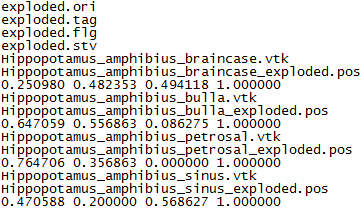
\includegraphics[scale=0.5]{images/07/project/ntw.png}
 \captionof{figure}{Example of project .ntw file containing references to orientation labels, tags labels and colors, flags and landmarks files.}
\label{project_file}
\end{figure}

\subsection{Open project}
Loads a .ntw file

\subsection{Save project}
\begin{figure}
  \centering  
 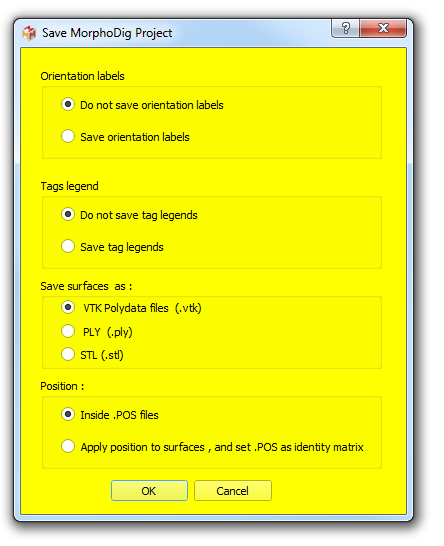
\includegraphics[scale=0.5]{images/07/project/save_ntw.png}
 \captionof{figure}{Save project window.}
\label{save_project_file}
\end{figure}
Behavior: only selected elements (surface objects, landmarks, flags...) are saved within projects. If at least one opened element has been selected, the Save project window (Fig. \ref{save_project_file} p.\pageref{save_project_file}) opens and asks whether :  
\begin{itemize}
\item orientation labels should be saved along with the project (by default, orientation labels are not saved, as orientation labels are quite rarely set by users). 
\item tag legends and colors (tag maps) should by saved. By default, .tag file are not saved along with the project, as tag setting is not a common task. 
\item save surfaces as. VTK polydata or PLY. We advise you to save your surfaces as VTK polydata. In the contrary cases scalar,  tag arrays and all RGB arrays having a name different from "RGB" will be lost.
\item save position inside .POS file, or apply the position to surfaces. We advise you to save position inside .POS file (otherwise, the initial orientations of your surfaces will be lost). 
\end{itemize}
Each surface file will be given the name of the original file. Each position file will be given a name which starts with the name of the associated surface and ends with the name of the project (1 exception: when the project contains only one surface and  the project's name is the same as that of the surface. In that case, .pos file names are not postfixed with the name of the project). In the .ntw file example shown in Fig. \ref{project_file} p.\pageref{project_file}, the surface files are 
\begin{itemize}
\item ``Hippopotamus\_amphibius\_braincase.vtk" 
\item ``Hippopotamus\_amphibius\_bulla.vtk" 
\item ``Hippopotamus\_amphibius\_petrosal.vtk" 
\item ``Hippopotamus\_amphibius\_sinus.vtk" 
\end{itemize}
\noindent and the project name is ``exploded.ntw". The advantage of naming position files that way is you may construct different .ntw files with different associated surface files using a same set of surfaces. Requirement : all selected surfaces saved via this option
need to have distinct names. Note : When working with ``project" files, if several surface objects have the same name, you may need at
some point to rename some of the object surfaces in order to make sure that all surface objects have a distinct name. To do so, select one surface, click on 
\includegraphics[scale=0.7]{images/06/objects/actor_edit.png}: the ``Edit first selected surface" window appears (See Fig. \ref{actor_edit} p.\pageref{actor_edit} in preceding chapter).




\section{Surface}
\subsection{Open surface}
STL, PLY and VTK polydata surfaces can be open via this menu. MorphoDig does not manage textures associated with surface files. When opening a PLY file containing RGB colors (for instance a file painted manually or automatically with ``MeshLab", or some laser scanner surface files) or a VTK file containing RGB arrays, these colors are placed inside a (or several) "RGB" array(s). 
%MorphoDig will reinitialize the ``RGB" scalars whenever you change the object's color or whenever you activate tag display mode or scalar display mode : if these colors are important to you, you may convert them to TAG values in the menu Tags$\rightarrow$Convert RGB colors to tags before changing the object color or display mode/before changing tags or any color scale activated.

\subsection{Save surface}
Selected surfaces can be saved into files. If no surface is selected, the following message appears:\\
\includegraphics[scale=0.5]{images/07/surface/no_surface_selected.png}\\
If at least 2 surfaces are selected, the following message shows up:\\
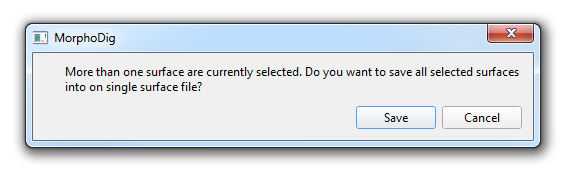
\includegraphics[scale=0.5]{images/07/surface/at_least_2_surfaces_selected.png}

\subsubsection{Save selected surfaces in one single .PLY file}

\begin{minipage}{0.5\textwidth}
Options:
\begin{itemize}
\item File type: you can save .ply data in binary (little or big endian)
or ASCII formats.
\item Position : you can keep object original coordinate system or
save the surface in its current position.
\item Normals : you can chose whether you wish to save normals.
\item Colors : RGB information associated to each vertex can be saved. You may decide either to keep current RGB color array (if that array exists). Alternatively, you may decide not to save the current RGB color array (if it exists). Finally, you may prefer to save/replace the current RGB color array as the current display color.
\end{itemize}

\end{minipage}    
\begin{minipage}{0.5\textwidth}\centering
  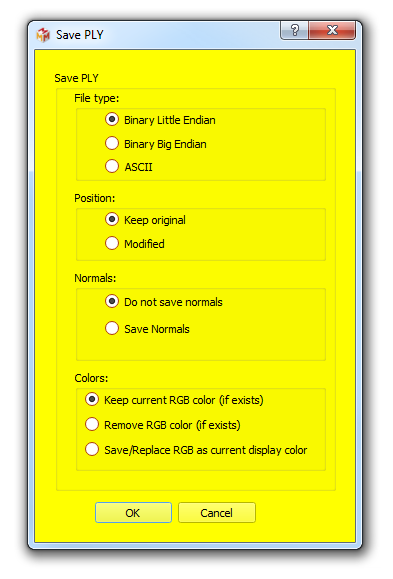
\includegraphics[scale=0.45]{images/07/surface/save_ply.png}
 \captionof{figure}{PLY save options window}
 \end{minipage} 

Note that a "RGB" array (object rendering color, depending on which rendering mode you
are using), depending on the chosen options, can be saved inside the .ply file. This means that Tag / Scalar / Object solid color can be exported and viewed in other software such as MeshLab.


\subsubsection{Save selected surfaces in one single .VTK PolyData (.VTK or .VTP) file}
\begin{minipage}{0.5\textwidth}
VTK polydata surface file format is by far not as widespread as STL or PLY
formats. However, it is extremely useful as it allows to store several
scalar, tag and RGB arrays.
Options:
\begin{itemize}
\item File type: you can save .VTK data in binary (little endian) or
ASCII formats.
\item Position : you can keep object original coordinate system
or save the surface in its current position.
\item Arrays: you decided which arrays (scalars, tags, RGB colors) should be saved inside the VTK polydata file.
\end{itemize}
\end{minipage}    
\begin{minipage}{0.5\textwidth}\centering
  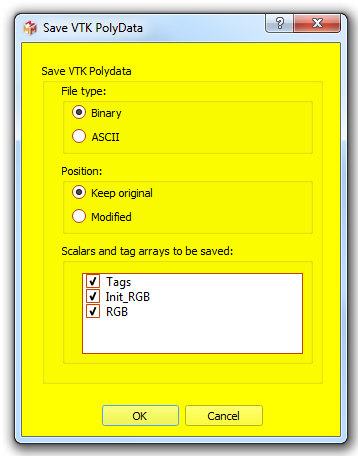
\includegraphics[scale=0.5]{images/07/surface/save_vtk.png}
 \captionof{figure}{VTK save options window}
 \end{minipage} 
\noindent


\subsubsection{Save selected surfaces in one single .STL file}

\begin{minipage}{0.5\textwidth}
Options:
\begin{itemize}
\item File type: you can save .stl data in binary (little endian) or
ASCII formats.

\item Position : you can keep object original coordinate system or save the surface in its current position
\end{itemize}

\end{minipage}    
\begin{minipage}{0.5\textwidth}\centering
  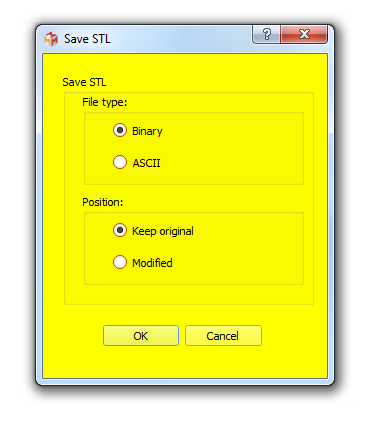
\includegraphics[scale=0.5]{images/07/surface/save_stl.png}
 \captionof{figure}{STL save options window}
 \end{minipage} 




\section{Position}
In MorphoDig, surface position consists in two
4*4 square matrices: the first matrix is currently not read nor used anymore by MorphoDig, but is kept for compatibility issues with older versions of MorphoDig and of ISE-MeshTools (MorphoDig is a major redesign of an older software, ISE-MeshTools). This first matrix will disappear in a near future.  The second matrix is the one that matters: the position matrix. It contains the rotation and translation information of 3D objects (3D surfaces and landmarks). These 2 matrices can be opened and saved in ``.pos" format (see Fig. \ref{position_file} p.\pageref{position_file}).


\begin{figure}
  \centering
  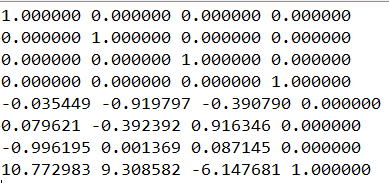
\includegraphics[scale=0.5]{images/07/position/position_file.png}
 \caption{Example of .pos position file. The first 4 lines correspond
to the aspect matrix, and the 4 last lines to the position matrix.}
\label{position_file}
\end{figure}
 



\subsection{Open position for selected surfaces}
If no surface is selected, the following message
appears:\\
\includegraphics[scale=0.5]{images/07/position/no_surface_selected.png}
\\
If at least 2 surfaces objects are selected, the same position will be given to them.

\subsection{Open transposed position for selected surfaces}
This option may be useful in the following case:
\begin{itemize}
\item Let us suppose that you did modify the position of a given surface and saved its position.
\item Then you have saved the surface in its current modified position (= the original position of the
surface is lost).
\end{itemize}

It may happen that you need to open the surface in its original position. To do so, you may apply this option (apply transposed position matrix to the modified surface).

\subsection{Open position for selected landmarks/flags}
If no landmark/flag is selected, the following message
appears:\\
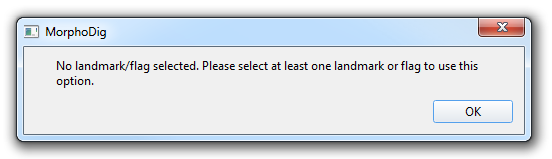
\includegraphics[scale=0.5]{images/07/position/no_landmark_selected.png}
\\
This options may be useful when you have digitized landmarks/flags on a given surface in its original position and orientation. Let us suppose that in a second step, you need to modify the position/orientation of that surface object and that you save it in a .POS file. You may then apply this .POS file to your set of landmarks/flags.

\subsection{Open transposed position for selected landmarks/flags}
If you have digitized landmarks/flags on a surface with a modified position (let us assume that the position of this surface is saved within a .POS file), by using this option, you can replace this landmarks/flags dataset on the surface in its original orientation. 


\subsection{Save position for selected surfaces}
Surface aspect and position matrices can be saved in ``.pos" format. If no surface is selected, the
following message appears:\\
\includegraphics[scale=0.5]{images/07/position/no_surface_selected.png}
\\
If at least 2 surfaces selected, the following message shows up:\\
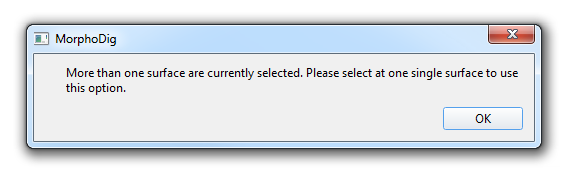
\includegraphics[scale=0.5]{images/07/position/at_least_2_surfaces_selected.png}

\subsection{Edit manually position matrix}
Clicking on "
\includegraphics[scale=0.7]{images/06/objects/actor_edit.png}" opens the "Edit first selected surface" window (Fig. \ref{actor_edit} p.\pageref{actor_edit}), in which the position matrix of a given actor can be modified.



\section{Landmarks}
Landmarks can be set on surfaces by pressing ``L" + left mouse click.\\

Two series of conventional landmarks can be set : ``normal" and ``target" landmarks. In the ``normal" landmark mode (button 
\includegraphics[scale=0.7]{images/04/normal_landmarks.png} active), pressing ``L" + left mouse click results in the creation a ``normal" landmark (a light green one). In the ``target" landmark mode (button 
\includegraphics[scale=0.7]{images/04/target_landmarks.png} active),
pressing ``L" + left mouse click will create a ``target" landmark (a yellow transparent one).

 ``Normal" and ``target" landmarks can be loaded and saved.\\
Selected landmarks can be reordered using the following buttons. Pressing ``
\includegraphics[scale=0.7]{images/06/objects/move_up.png}"
will (try to) increase the number of all selected landmarks, while pressing ````
\includegraphics[scale=0.7]{images/06/objects/move_down.png}""
will (try to) decrease their number, respectively.\\\\
MorphoDig can manage three types of landmark files: ``.LMK", ``.VER" and ``.STV" files.
\begin{itemize}
\item 
 .LMK files contain a series of lines, each line
being constructed the following way (see Fig. \ref{LMK_file} p.\pageref{LMK_file}): landmark
name (without space or tab character),
landmark coordinates. Note that each landmark name does not need to be of the form ``landmark"+landmark number. Meanwhile, the name should not hold space or tab
characters.
\item .VER files contain a series
of lines, each line being
constructed the following
way (see Fig. \ref{VER_file} p.\pageref{VER_file}): landmark name (without space or tab character), landmark coordinates, landmark orientation.
\item STV files may contain one or two series of line. The first line contains two integers, the first being the type of landmark (0 for ``normal" or 1 for ``target"), the second being the number of lines of landmarks of this type which are expected to follow, constructed the following way: landmark name (without space or tab character), landmark coordinates, landmark orientation. An example of .STV file containing both ``normal" and ``target" landmarks is given in Fig. \ref{STV_file} p.\pageref{STV_file}. Note that the number of ``normal" and ``target" landmarks saved within a .STV file can differ.
\end{itemize}
\begin{figure}
  \centering
  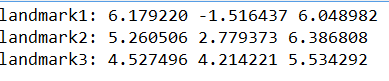
\includegraphics[scale=0.5]{images/07/landmarks/LMK_file.png}
 \caption{Example of .LMK file}
\label{LMK_file}
\end{figure}

\begin{figure}
  \centering
  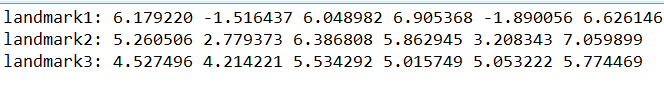
\includegraphics[scale=0.5]{images/07/landmarks/VER_file.png}
 \caption{Example of .VER file}
\label{VER_file}
\end{figure}
\begin{figure}
  \centering
  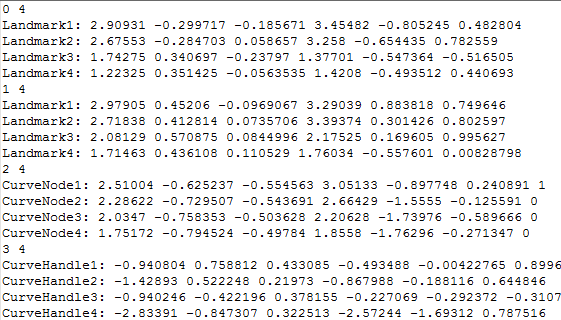
\includegraphics[scale=0.5]{images/07/landmarks/STV_file.png}
 \caption{Example of .STV file. We advise you to use this file format.}
\label{STV_file}
\end{figure}

\subsection{Open MorphoDig Landmark/Curve File (STV)}
STV file contain lists of "normal", "target" landmarks (but may also contain lists of "curve node" and "curve handle" landmarks).
\subsection{Open Landmarks}
Landmarks (.VER or .LMK) opened using this option will be put in the ``normal" landmark list (light green landmarks)
\subsection{Open Target Landmarks}
Landmarks opened using this option will be put in the ``target" landmark list (yellow transparent landmarks)
\subsection{Save MorphoDig Landmark/Curve File (STV)}
You may decide whether you wish to save all (normal, target, curve node, curve handle) landmarks or only selected ones (see Fig. \ref{save_stv} p.\pageref{save_stv}).
\begin{figure}
  \centering
  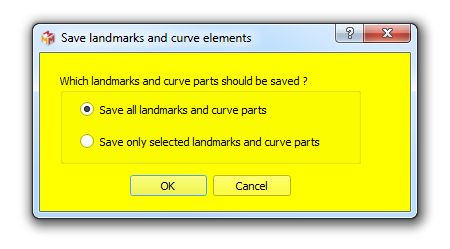
\includegraphics[scale=0.5]{images/07/landmarks/save_stv.png}
 \caption{Save STV window.}
\label{save_stv}
\end{figure}

\subsection{Save Landmarks}
You may decide whether you wish to save only selected ``normal" landmarks or all selected and
unselected ``normal" landmarks (the yellow transparent ones) in .VER or .LMK format (see Fig. \ref{save_ver_lmk} p.\pageref{save_ver_lmk}).
\begin{figure}
  \centering
  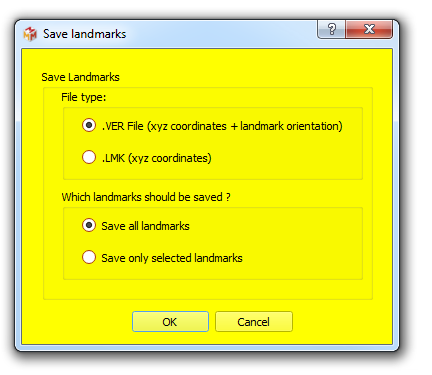
\includegraphics[scale=0.5]{images/07/landmarks/save_ver_lmk.png}
 \caption{Save Landmark Window. Used to save either "Normal", "Target" landmarks (but not both at the same time). This windows is also used to save curve nodes or curve handles in .LMK and .VER format (but also not both at the same time). }
\label{save_ver_lmk}
\end{figure}.
The ``Landmarks" chapter (chapter \ref{landmark_chapter} p.\pageref{landmark_chapter}) and the tutorial ``working with landmarks" contain further information regarding landmark digitization with MorphoDig.


\subsection{Save Target Landmarks}
You may decide whether you wish to save only selected ``target" landmarks or all selected and
unselected ``target" landmarks (the yellow transparent ones) in .VER or .LMK format (see Fig. \ref{save_ver_lmk} p.\pageref{save_ver_lmk}).
The ``Landmarks" chapter (chapter \ref{landmark_chapter} p.\pageref{landmark_chapter}) and the tutorial ``working with landmarks" contain further information regarding landmark digitization with MorphoDig


\section{Curves}\label{file_curve_section}

3D Curves (series of 3D cubic Bezier curves) are constructed in MorphoDig using 2 series of landmarks : a series of N ``curve node" landmarks, and a series of N ``curve handle".  Curve nodes and handles can be set on surfaces by pressing ``L" + left mouse click. In the ``curve nodes" landmark mode (button 
\includegraphics[scale=0.7]{images/04/curve_nodes.png} active), pressing ``L" + left mouse click results in the creation a ``curve node" landmark (a dark green for a curve starting node, and then light red ones). In the ``curve handles" landmark mode (button 
\includegraphics[scale=0.7]{images/04/curve_handles.png} active), pressing ``L" + left mouse click will create a ``target" landmark (a violet transparent one).

Selected curve nodes/handles can be reordered using the following buttons. Pressing ``
\includegraphics[scale=0.7]{images/06/objects/move_up.png}"
will (try to) increase the number of all selected curve nodes/handles, while pressing ````
\includegraphics[scale=0.7]{images/06/objects/move_down.png}""
will (try to) decrease curve nodes/handles number, respectively.\\


3D Bezier curves passing through all curve nodes are draw green when no curve node/handle belonging to
the curve segment is selected. Curves are drawn red when at least one curve node/handle involved in the
curve segment is selected. Two different cases are considered:
\begin{itemize}

\item Case 1: the numbers of ``curve node" and ``curve handle" landmarks differ. In that case, a curve is a series of lines passing through ``curve node" landmarks.
\item Case 2: the numbers of ``curve node" and ``curve handle" landmarks are equal. In that case, a curve is a
series of cubic Bezier curves passing through ``normal" landmarks. For a given set of 2 ``curve node"
consecutive landmarks (Ln and Ln+1) and their associated ``curve handles" (Hn and Hn+1), a mirror
image of Hn+1 relative to Ln+1 (H'n+1) is constructed. The Bezier curve involving Ln, Ln+1, Hn and
Hn+1 starts from Ln, going toward Hn, and arrives at Ln+1 coming from the direction of H'n+1.

\end{itemize}


The explicit form of the curve is :
\begin{equation}
B(t) = (1-t)^{3}Ln + 3(1-t)^{3}tHn + 3(1-t)t^{2}H'n+1 +t^{3}Ln+1, t \in[0,1]
\end{equation}
\\
In order to be able to digitize several curves using a given set of curve node and curve handle landmarks,
``curve node" landmarks curves can be given 4 flags (see section \ref{landmarks_curves_section} p.\pageref{landmarks_curves_section} ``Landmarks $\rightarrow$ selected curve node and handle landmarks" for further details):\\
Flag ``0" : node is within a given curve segment (drawn ``red").\\
Flag ``1" : node is the starting point of a curve segment (drawn dark ``green").\\
Flag ``2" : node is placed inside the curve, and is a curve ``milestone" (drawn blue) .\\
Flag ``3" : node is placed inside the curve, and should be connected to the preceding curve
segment starting point. When curve node "N" is flagged that way, curve node "N+1" will be set automatically as a curve segment starting point.\\
Flag ``2" is used to decompose a given curve segment into curve sub-segments. By default, a curve comprises 1 segment.\\
Flag ``3" is used to close a curve (by default, curves are open).\\
3D curves are loaded and saved into either .STV (more generic) or .CUR (more specific) files. CUR files which contain a series of lines, each line being
constructed the following way: name (without space or tab character), curve ``node" landmark
coordinates, curve ``handle" coordinates, flag.
In the example shown below, 4 curves are defined :\\
- an open curve starting from curve node 1 and ending at landmark 7\\
- a closed curve involving landmarks 8 to 12\\
- an open curve involving landmarks 13 to 20\\
- a closed curve involving landmarks 21 to 26\\
These four curves contain only one sub-segment (no curve milestone was set within those 4 curves).
Note that each name does not need to be of the form ``CurvePart"+ number. Meanwhile, the name
should not hold space or tab characters.
\begin{figure}[t] 
  \centering
  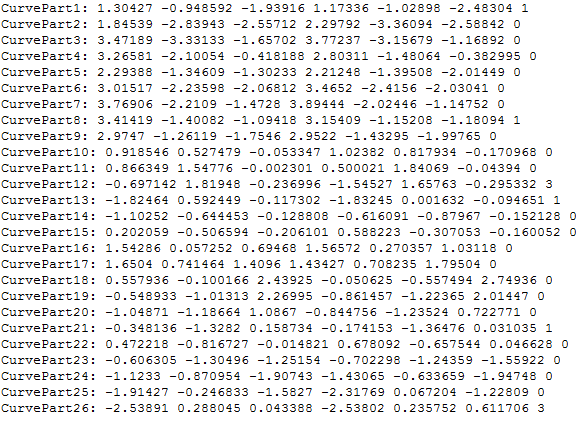
\includegraphics[scale=0.5]{images/07/curves/CUR_file.png} 
	\caption{Example of .CUR file}
 
\end{figure}

\subsection{Open Curve (.CUR)}
This menu allows the user to load a .CUR file.
\subsection{Open MorphoDig Landmark/Curve file (.STV)}
This menu allows the user to load a STV file, as STF files can contain lists of curve node and curve handle landmarks (see for instance Fig. \ref{STV_file} p.\pageref{STV_file}).
\subsection{Open Curve Node Landmarks}
This menu allows the user place the content of a VER or LMK file inside the list of curve node landmarks.
\subsection{Open Curve Handle Landmarks}
This menu allows the user place the content of a VER or LMK file inside the list of curve handle landmarks.
\subsection{Save .CUR file}
This menu allows the user to save current landmarks and curve handles as a .CUR file. This action is only allowed if the number of ``curve node" landmarks and ``curve handle" landmarks is the same. If not, the following message appears:\\
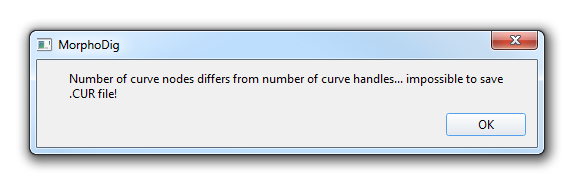
\includegraphics[scale=0.5]{images/07/curves/nnodes_nhandles_differ.png}
\\
If you are in the process of digitizing curves (and do not have achieved to digitize the same number of ``normal" and ``target"  landmarks and wish to save the current state of your work, you may decide to save curve node and target landmarks within a STV file instead (see next section ).
\subsection{Save MorphoDig Landmark/Curve File (STV)}
You may decide whether you wish to save all curve node and curve handle landmarks or only selected ones (see Fig. \ref{save_stv} p.\pageref{save_stv}). Using this option will also save "normal" and "target" landmark lists.
\subsection{Save Curve Node Landmarks}
Curve node landmarks can be saved inside a LMK or VER file using this option. You may decide whether you wish to save only selected ``curve node" landmarks or all selected and unselected ``curve node" landmarks in .VER or .LMK format (see Fig. \ref{save_ver_lmk} p.\pageref{save_ver_lmk}).

\subsection{Save Curve Handle Landmarks}
Curve handle landmarks can be saved inside a LMK or VER file using this option. You may decide whether you wish to save only selected ``curve handle" landmarks or all selected and unselected ``curve handle" landmarks in .VER or .LMK format (see Fig. \ref{save_ver_lmk} p.\pageref{save_ver_lmk}).


\subsection{Export Curves as Landmark file}
\begin{minipage}{0.55\textwidth}

Curves can be transformed in a series of equidistant landmarks using this option. The curve decimation window
appears.
Each curve \textbf{segment} is saved as a number of
equidistant landmarks.\\
Be aware that there are two ways to define curve \textbf{segments} in MorphoDig : \\
- by setting curve node "starting points" , in order to create \textbf{independent} curve segments (see section \ref{section_curve_segment1} p.\pageref{section_curve_segment1}, and a practical example Fig. \ref{starting_node} p. \pageref{starting_node})\\
- by setting curve node "milestones", in order to create \textbf{contiguous} curve segments (see section \ref{section_curve_segment2} p.\pageref{section_curve_segment2}, and a practical example Fig. \ref{curve_milestone} p. \pageref{curve_milestone}).
\\
 You may also decide to save normal and target landmarks information inside the VER or LMK output. This is useful when you need to use both type 1 landmarks (normal and target landmarks) and semi-landmards (3D curves) in Geometric Morphometric analyses. 

In the present example, each curve/
curve segment is saved as 20 equidistant landmarks.

\end{minipage}  
 \begin{minipage}{0.45\textwidth}\centering
  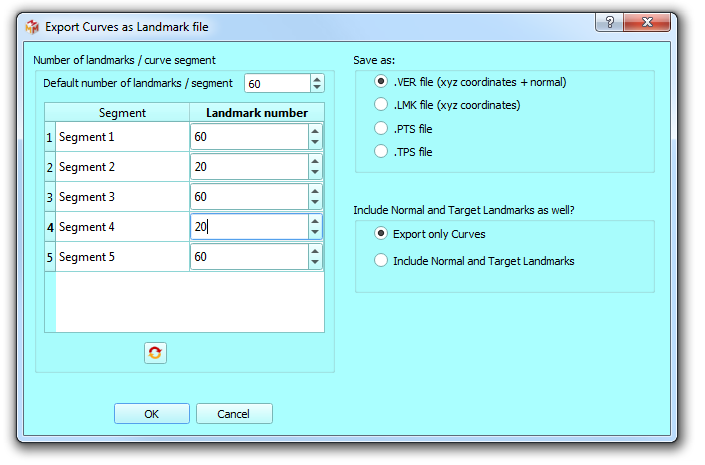
\includegraphics[scale=0.5]{images/07/curves/export.png}
 \captionof{figure}{Export curves as landmark file window}
 \end{minipage} 



\subsection{Save curve infos (length per curve segment)}
\begin{minipage}{0.55\textwidth}

Each curve \textbf{segment} length can be saved as a .txt file using this option. 
As stated in the preceding section, we want to insist on the fact that there are two ways to define curve \textbf{segments} in MorphoDig : \\
- by setting curve node "starting points" , in order to create \textbf{independent} curve segments (see section \ref{section_curve_segment1} p.\pageref{section_curve_segment1}, and a practical example Fig. \ref{starting_node} p. \pageref{starting_node})\\
- by setting curve node "milestones", in order to create \textbf{contiguous} curve segments (see section \ref{section_curve_segment2} p.\pageref{section_curve_segment2}, and a practical example Fig. \ref{curve_milestone} p. \pageref{curve_milestone}).\\

The ``Landmarks" chapter (chapter \ref{landmark_chapter} p.\pageref{landmark_chapter}) and the
tutorial ``Working with curves" contain further important
information regarding curve digitization with MorphoDig.

\end{minipage}  
 \begin{minipage}{0.45\textwidth}\centering
  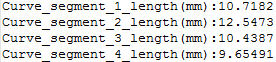
\includegraphics[scale=0.5]{images/07/curves/Curve_infos.png}
 \captionof{figure}{Example of curve info file}
 \end{minipage} 

\section{Flags}

Regarding flags, as stated earlier, one series of ``flag landmarks" can be digitized in MorphoDig (button `
\includegraphics[scale=0.7]{images/04/flag_landmarks.png}" should
be pressed). To edit flag label, length and color, select one
flag landmark, click on "
\includegraphics[scale=0.7]{images/06/objects/flag_edit.png}" in order to open the "Edit first selected landmark" window (Fig. \ref{flag_edit} p.\pageref{flag_edit}). Pressing ok will update the label, the color and the length associated to the selected flag, which in turn will be unselected. 

\noindent
Flags are saved using the .FLG file format, which consists of n pairs of lines constructed the following way (Fig. \ref{FLG_file} p.\pageref{FLG_file}):\\
line 2*n: Flag name\\
line 2*n+1: Flag coordinates, flag orientation, flag length and color.

\begin{figure}
  \centering
  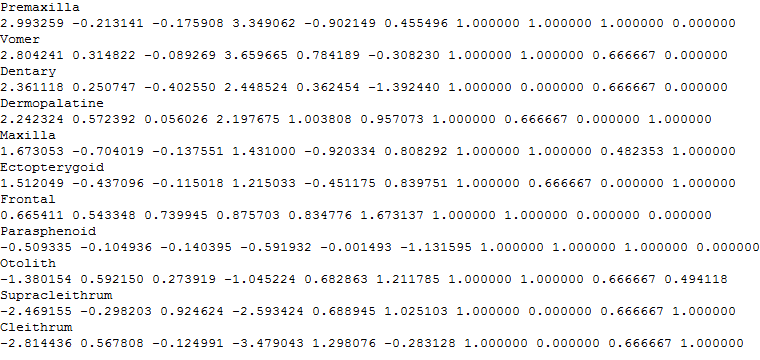
\includegraphics[scale=0.5]{images/07/flags/FLG_file.png}
 \caption{Example of .FLG file}
\label{FLG_file}
\end{figure}

\subsection{Load flags}
Select a .FLG file using this menu

\subsection{Save flags}
This option saves the current flag landmarks into a .FLG file, regardless their selection status.


\section{Color maps}


- Color maps are used to visualize scalar arrays (=arrays of numbers associated to each vertex) and can be edited interactively by
clicking on 
\includegraphics[scale=0.7]{images/07/colormaps/colormaps.png}, which opens the "Scalar rendering options" window (see chapter
``Scalars" (chapter \ref{scalars_chapter} p.\pageref{scalars_chapter}) and the tutorial ``Working with scalars" for
further information).\\
- Scalars become visible when the array display mode button is pressed (
\includegraphics[scale=0.7]{images/04/show_color_scale.png}), and a scalar array is selected (ex:
\includegraphics[scale=0.5]{images/04/scalarcombo_scalar.png}).\\
Two default color maps exist in MorphoDig, which can be edited, but not deleted : the "Rainbow" the "Black-Red-White" color maps. Any number of additional color maps can be added to the list of existing color maps, and are referred to as "custom color maps".


An example of color map (.MAP) file and how it translates into an actual color/opacity map is shown Fig. \ref{color_map_example} p.\pageref{color_map_example}):\\

\begin{figure}
  \centering
  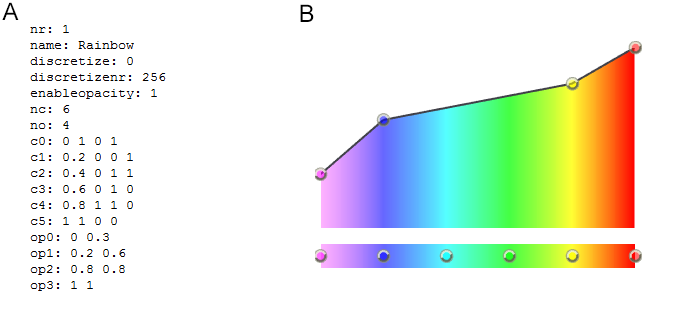
\includegraphics[scale=0.5]{images/07/colormaps/example.png}
 \caption{A. Example of .MAP file containing one single colormap named "Rainbow", and having 5 color and 4 opacity control points. B. Translation of this colormap inside MorphoDig.}
\label{color_map_example}
\end{figure}


\subsection{Import color maps (.MAP)}
Imports one or several color maps included inside a .MAP file. 

\subsection{Export color maps (.MAP)}

\begin{minipage}{0.55\textwidth}
This option opens the Export color maps window, in which the active color map, all color maps (the 2 default color maps + all custom color maps), or all custom color maps can be saved inside a .MAP file.


\end{minipage}  
 \begin{minipage}{0.45\textwidth}\centering
  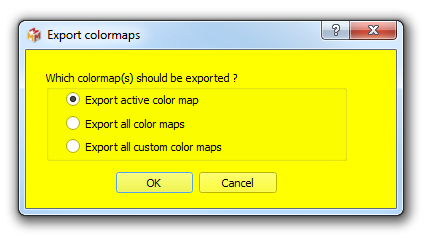
\includegraphics[scale=0.5]{images/07/colormaps/export.png}
 \captionof{figure}{Export color maps window.}
 \end{minipage} 


\section{Tag maps}


- Tag colors and names (=tag maps) can be edited interactively by
clicking on 
\includegraphics[scale=0.7]{images/07/tagmaps/tagmaps.png}, which opens the Tags window (see the chapter
``Tags" (chapter \ref{tags_chapter} p.\pageref{tags_chapter}) and the tutorial ``Working with tags" for
further information).\\
- Tags become visible when the array display mode button is pressed (
\includegraphics[scale=0.7]{images/04/show_color_scale.png}), and a tag array is selected (ex:
\includegraphics[scale=0.5]{images/04/scalarcombo_tag.png}).

Tag maps consist mostly of a series of combination of a tag name and an associated color.  Any number of tag name + color can be defined (25 different names+colors by default, but this number can be interactively increased/decreased).\\
By default, MorphoDig contains one Tag maps named "TagMap", which can not be deleted, but can be edited as needed. Other tag maps can be added manually to tag map list, and are referred to as "custom tag maps". 


Tag map files come in two formats : .TAG and .TGP.

\begin{minipage}{0.55\textwidth}
TAG format consists of N pairs of lines, can store one single tag map, and is constructed the following way:
line 2*n: Tag name\\
line 2*n+1: Tag color and transparency
\end{minipage}  
 \begin{minipage}{0.45\textwidth}\centering
  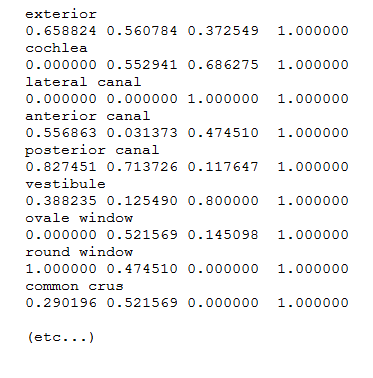
\includegraphics[scale=0.5]{images/07/tagmaps/TAG_file.png}
 \captionof{figure}{Example of .TAG file}
 \end{minipage} 

\noindent

\begin{minipage}{0.55\textwidth}
TGP format differs from TAG in that it can store several tag maps and gives a name to each tag map. An example of TGP file containing 2 tag maps is shown aside.\\
line 2*n: Tag name\\
line 2*n+1: Tag color and transparency
\end{minipage}  
 \begin{minipage}{0.45\textwidth}\centering
  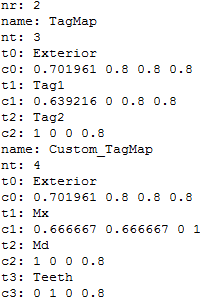
\includegraphics[scale=0.5]{images/07/tagmaps/TGP_file.png}
 \captionof{figure}{Example of .TGP file containing two tag maps. The first contains 3 entries, the second 4 entries. }
 \end{minipage} 

\noindent



\subsection{Import tag maps (.TGP or .TAG)}
Imports one tag map (.TAG or .TGP file) or several tag maps (.TGP file). Then open the tag window (click on 
\includegraphics[scale=0.7]{images/07/tagmaps/tagmaps.png}) : Tag labels, colors and transparencies should have been updated. In the "Tags window", you can switch between different tag maps with the combo box "Chose tag map".

\subsection{Export tag maps (.TGP or .TAG)}

\begin{minipage}{0.55\textwidth}
This option opens the Export tag maps window, in which the active tag map, all tag maps (= default tag map + all custom tag maps), or all custom tag maps can be saved inside either a .TAG file (if only one tag map should be saved) or inside a .TGP file (one or several tag maps).


\end{minipage}  
 \begin{minipage}{0.45\textwidth}\centering
  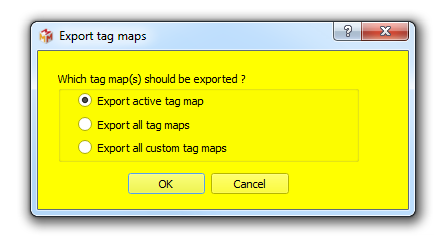
\includegraphics[scale=0.5]{images/07/tagmaps/export.png}
 \captionof{figure}{Export tag maps window.}
 \end{minipage} 

\section{Orientation helper labels}
The coordinate system orientation helper labels can be saved into ``.ORI" files, which are .txt files
containing 6 lines, 1 for each axis.


\subsection{Open Orientation labels}
Select a .ORI file using this menu.  Then open the orientation labels window window (Edit$\rightarrow$Edit 
Orientation labels) : the 6 orientation labels should have been updated.

\subsection{Save Orientation labels}
This option saves the current state of orientation labels in a .ORI file.

\section{Measurements}
\subsection{Save area, volume, triangle number and vertex number of selected surfaces}
\noindent
Surface area, volume, triangle number and vertex number of all selected surface objects can be saved in a .txt file using this option.\\
\noindent Note: surface objects should be closed in order to provide a correct estimation of object volume.

\subsection{Complexity: save normalized shape index, area and volume of selected surfaces} \label{global_complexity_1}
\noindent
Surface normalized shape index (NSI) can be viewed as a measurement of surface "complexity" (= how much area can be enclosed within a given volume). Surface normalized shape index (NSI), surface area and surface volume of all selected surface objects can be saved in a .txt file using this option.\\
For a given surface of area "SA" and of volume "V", "NSI" is a measurement of how much the ratio between surface area and surface volume differs from that of a sphere. It is defined as: 

\begin{equation}
NSI = F \dfrac{\sqrt[2](SA)}{\sqrt[3](V)}
\end{equation}

where F is a constant defined so that perfectly spherical 3D surfaces express a NSI index equal to 1, and higher values for non spherical shapes:
\begin{equation}
F = \dfrac{\sqrt[3](\dfrac{4}{3}\pi)}{2\sqrt[2](\pi)}
\end{equation}

\subsection{Complexity: save convex hull area ratio and convex hull normalized shape index of selected surfaces (warning: slow).} \label{global_complexity_2}
\noindent
Surface normalized shape index (NSI, see preceding section) may not offer a good estimate of "global shape complexity" of surfaces, especially when surfaces' shape differ very much from that of a sphere (very flat objects).  
Other metrics, such as Convex hull area ratio (ChAR), or convex hull normalized shape index (ChNSI), may be better proxies for a global measurements of shape complexity for whole surfaces (= how much area can be enclosed within a given volume). 
 ChAR, ChNSI and surface area, surface volume, convex hull, convex hull volume and surface normalized shape index (NSI: defined in the preceding section) of all selected surface objects can be saved in a .txt file using this option.\\

\subsubsection{ChAR}

\noindent For a given surface of area "SA", ChAR is the ratio between "SA" and the surface area of the convex hull of that same surface (ChSA). Its aim is to compare the surface area of a surface with that of that of a "wrapping bag" that would enclose that surface. It is defined as: 


\begin{equation}
ChAR = \dfrac{SA}{ChSA}
\end{equation}

\noindent Perfectly spherical 3D surfaces express a ChSA index equal to 1 while, while hihly folded structures (such as turbinates)  usually express values higher than 1. Shapes spread in space and containing a lot of holes may express ChSA values smaller than 1.

\subsubsection{ChNSI}
\noindent For a given surface of area "SA" and of volume "V", "ChNSI" measures how much surface area "SA" can be enclosed within the volume of the convex hull ("ChV") computed for that same surface It is defined as: 

\begin{equation}
ChNSI = F \dfrac{\sqrt[2](SA)}{\sqrt[3](ChV)}
\end{equation}

\noindent where F is a constant defined so that perfectly spherical 3D surfaces express a ChNSI index equal to 1 :
\begin{equation}
F = \dfrac{\sqrt[3](\dfrac{4}{3}\pi)}{2\sqrt[2](\pi)}
\end{equation}

\noindent Perfectly spherical 3D surfaces express a ChNSI index equal to 1. Hihly folded structures (such as turbinates) usually express ChNSI values higher than 1. Shapes spread in space and containing a lot of holes may express ChSA values smaller than 1.

\subsection{Save size measurements (max length in xyz direction etc.) of all selected surfaces.}
Depending on your biological scientific question, you may need different measurements of the "size" of your structure of interes. This menu provides different "size metrics" for 3D surfaces which can be relevant. \\
\subsubsection{Bounding box length}
Bounding box length gives an idea of the maximal length of a 3D surface. However, this metrics depends on the orientation of the surface, so be careful when using it.

\subsubsection{Mean and maximal distances to centroid}
For a given surface containing N vertices, the centroid is defined as the average x,y,z coordinates of all N vertices. The mean distance of all N vertices to the centroid, and the maximal distance for all N vertices to the centroid give information regarding the expansion in 3D space of your structure.
\subsubsection{PC1, PC2, PC3 length and average of PC1, PC2, PC3}
A better alternative to the bounding box length metrics is as follows: for a given surface, MorphoDig computes a Principal Component Analysis (PCA) of all 3D vertex coordinates. Then all vertices are projected on Principal component 1 (PC1), on PC2 and on PC3. The difference between the maximal projection scores and minimal projection scores on a given PC give the length of your structure of interest along that axis. PC1 length is a measurement of the maximal length of your structure. PC2 and PC3 lengths are measurements of the maximal width and height of your structure. PC1, PC2 and PC3 length do not depend on 3D surface orientation and are in that sense much reliable metrics than bounding box length. 

\subsection{Save active scalar infos (mean, median, variance ...) of all selected surfaces.}
In order to use this option, the array display mode button must be pressed (
\includegraphics[scale=0.7]{images/04/show_color_scale.png}), and a scalar array must also be selected selected (ex:
\includegraphics[scale=0.5]{images/04/scalarcombo_scalar.png}).\\
This option saves within a .txt file, and for all selected surfaces, the mean, the median, and the variance of the selected scalar.

\subsection{Save scalar values of first selected surface.}
This option saves within a .txt file, and ONLY for the first selected surface containing N vertices, all scalar values for all vertices. Ex: if a given surface contains 3 scalars (ex: thickness, curvature, complexity), the .txt file will contain the values of the 3 scalar arrays for all N vertices. 